
% -------------------------------------------------------------------------------
% Preamble
% -------------------------------------------------------------------------------
\documentclass[paper=a4, fontsize=11pt,twoside, bibliography=totoc]{scrartcl}		% KOMA article

\ifx\pdftexversion\undefined
\usepackage[dvips]{graphicx}
\else
\usepackage[pdftex]{graphicx}
\DeclareGraphicsRule{*}{mps}{*}{}
\fi

\usepackage[a4paper,pdftex]{geometry}										% A4paper margins
\setlength{\oddsidemargin}{5mm}												% Remove 'twosided' indentation
\setlength{\evensidemargin}{5mm}

\usepackage{xspace} % Define commands that don't eat spaces.
\usepackage[english]{babel}
\usepackage[protrusion=true,expansion=true]{microtype}	
\usepackage{amsmath,amsfonts,amsthm,amssymb}
\usepackage{graphicx}



%% Captions (Schrift, Aussehen) ==========================================

%%% Doc: ftp://tug.ctan.org/pub/tex-archive/macros/latex/contrib/caption/caption.pdf
\usepackage{caption}
% Aussehen der Captions
\captionsetup{
   margin = 10pt,
   font = {small,rm},
   labelfont = {small,bf},
   format = plain, % oder 'hang'
   indention = 0em,   % Einruecken der Beschriftung
   labelsep = colon, %period, space, quad, newline
   justification = RaggedRight, % justified, centering
   singlelinecheck = true, % false (true=bei einer Zeile immer zentrieren)
   position = bottom %top
}
%%% Bugfix Workaround
\DeclareCaptionOption{parskip}[]{}
\DeclareCaptionOption{parindent}[]{}

% Aussehen der Captions fuer subfigures (subfig-Paket)
\captionsetup[subfloat]{%
   margin = 10pt,
   font = {small,rm},
   labelfont = {small,bf},
   format = plain, % oder 'hang'
   indention = 0em,   % Einruecken der Beschriftung
   labelsep = space, %period, space, quad, newline
   justification = RaggedRight, % justified, centering
   singlelinecheck = true, % false (true=bei einer Zeile immer zentrieren)
   position = bottom, %top
   labelformat = parens % simple, empty % Wie die Bezeichnung gesetzt wird
 }

% ------------------------------------------------------------------------------
% Definitions
% ------------------------------------------------------------------------------
\newcommand{\HRule}[1]{\rule{\linewidth}{#1}} 	% Horizontal rule

\newcommand{\wms}{\emph{Elevated WMS}\xspace}
\newcommand{\sud}{\emph{Sudplan3D}\xspace}

\makeatletter							% Title
\def\printtitle{%						
    {\centering \@title\par}}
\makeatother									

\makeatletter							% Author
\def\printauthor{%					
    {\centering \large \@author}}				
\makeatother							
\begin{document}
\section{Covida}
Annotating videos is an exhausting task, but it has a great benefit for several communities. 
Thus labeled ground truth data is the foundation for supervised machine learning approaches. 
Covida offers an easy accessible interface for annotating video data in single user enviroment, for example Asus EEE Slate, and multi user enviroment, like collaborative work on a pen enabled multi touch table.
\par
\label{sec:intro}
\begin{figure}[!ht]
\captionsetup{type=figure} 
 \centering
 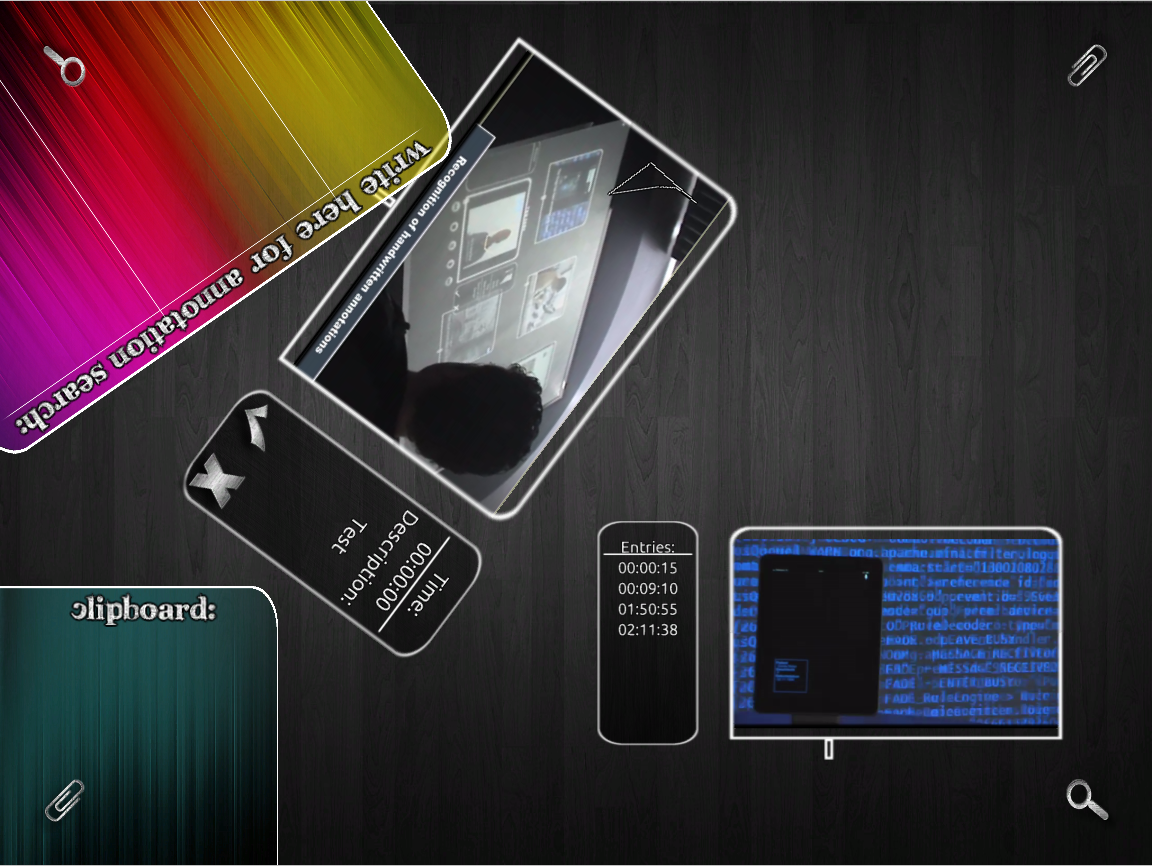
\includegraphics[width=.85\columnwidth]{screenshot}
 \caption{Covida screenshot.}
 \label{fig:overview1}
\end{figure}
Figure~\ref{fig:overview1} introduces the interface of the key features provided by Covida.
Covida offers the possibility to annotate videos directly via touch gestures, drawings and handwriting.
For outlining and labeling the shape of an object, Covida provides a pen-based interface which combines pen and touch input. 
User studies showed that especially for complex structures the usage of a pen device improves the effectiveness of the outlining process.
Annotations can be searched via handwritings on the search field (See Figure~\ref{fig:overview1} upper left corner) which can easily be accessed via touch gestures.
Further annotation text can be stored in the clipboard (See Figure~\ref{fig:overview1} bottom left corner) via dragging of the annotation text via touch drag gestures.
In a similar way annotations can be assigned to semantic groups like a name of a person to the semantic group 'person'.
Further the stored annotation data is saved as aRDF data in a XML file to grant the possibilty to modify and visualize the labled annotation data outside of the Covida application.

\end{document}